\chapter{Introduction}
I am glad to work with Algonauts Technologies Pvt. Ltd. as a Software Developer. This opportunity gave me hands-on experience in project planning,  database designing, and UI development, Could based environment, generating statistics \& parameter optimization. I also got a chance to showcase my skills with ease to adapt and modify the project with a change in business, or user requirements.\\

My work encompasses around : 
\begin{itemize}
\item Designing the web-based software modules with a simple \& sleek user interface.
\item Developing and maintaining backend for website
\item Integrating the online payment for enlarging subscription support.
\item Deploying project on Azure Cloud Environment.
\item Deriving various insightful parameters using statistics \& visualization
\item Developing Trade calls Dashboards for stock prices and calls rendering
\end{itemize}

\section{Algonauts Technologies Pvt. Ltd.}
In a nutshell, Algonauts Technologies Pvt. Ltd. deals with the financial spectrum under which it specializes in Algorithmic Trading in Indian Stock Market. The Founders have a vast experience of about 20 years in dealing with Stock Market, Finance, handling portfolios of HNIs, Algo-Trading, etc.
Currently, the company has products that involve mathematical \& statistical algorithms for stock price prediction \& subsequently a buy/sell stock call generator.
These products incorporate well-renowned stock market indicators such as MA, MACD,  Super-Trend, etc.  
The product serves all kinds of trades such as IntraDay, BTST, Positional, and Longterm.
\par

\section{Location of Internship}
% $<$Add office location and team details here$>$\newline
The office is located at 20, 2nd Floor, SP-TBI, RPI Building, Next to Bhavans College Main Gate, Munshi Nagar, Andheri West, Mumbai 400053.
My Team comprised of  Back end Developer Intern, UI/UX Design Intern, one supervisor \& two Managers.
\par

\section{Project Description}
\textbf{Background}\\

Mercury, a product designed to serve the Traders/ Clients for placing an efficient and accurate BUY/SELL call for the instrument. 
Here ``instrument" refers to Stock Name in the NSE market. 
The client/trader can choose to trade in Intra Day, BTST, Positional \& longterm. 
The Orders are placed via Kite API by Zerodha that provides real-time order placement towards Stock Exchange.
This product was initially a standalone application that had less scalability. Owing to this multiple advancements are added which are mentioned in the following. 
\par
The main aim is to modernize this application \& re-engineer to create a business-subscription model. In addition to this, Fast \& reliable service, Security compliance, and simple \& sleek UI are the major avenues to be developed. The product also involves customizing the trade calls based on preference, with options to customize every little thing, from web notification to user-based filters.
\begin{figure}[ht]
\centering
\scalebox{0.5}{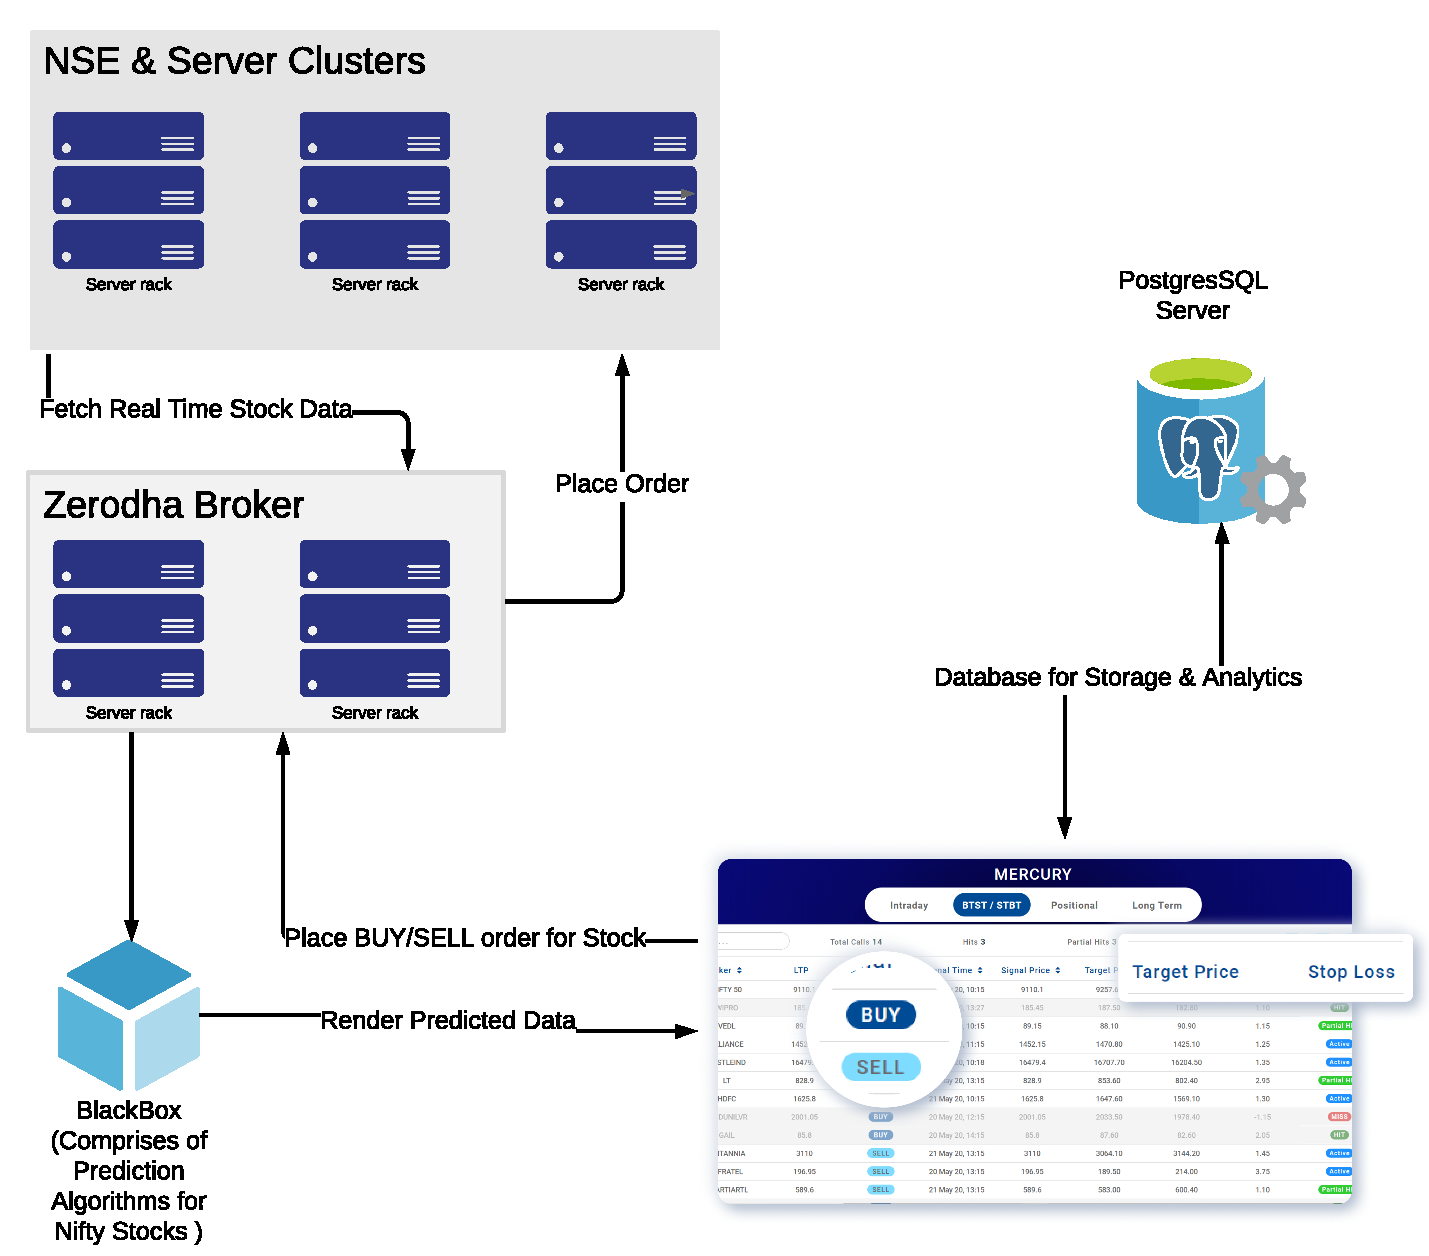
\includegraphics{algo_project.pdf}}
\caption{Product Overview}
\label{vmb}
\end{figure}


\subsubsection{Django}

For web development Django act as backend for website. Django Framework which is a high-level Python Web framework that encourages rapid development and clean pragmatic design. Django provides various library support to configure the project to API mode, along with UI built, using jinja templating. Jinja is a modern and designer-friendly templating language for Python, which renders web pages on the server-side. Django also has pre-built support for Postgres Database Engine. 

\subsubsection{PostgreSQL}
PostgreSQL is the primary database engine used in whole Algonauts system. PostgreSQL is a general-purpose and object-relational database management system, the most advanced open-source database system. It is incorporated due to its performance \& ACID compliance which is an essential need for any modern web-based product. Postgres, provide \textit{User Defined Type} which is one of the most advance and essential feature while developing any modern application which makes database object-oriented. It also provides Multiversion Concurrency Control (MVCC) support which always keeps data consistent.

\subsubsection{Redis \& Daphne}
\textbf{Redis} is an open-source, in-memory data store, used as a database cache and message broker. It forms channels and groups to cache the message. This creates Pub/Sub architecture, where messages are delivered on a subscription basis. Channel is mapped to a specific route, and groups are made to categorize the message and restrict message delivery for user subscription, making a robust dynamic business subscription model for the product.  \textbf{Daphne} is an HTTP,  and WebSocket protocol server for ASGI and ASGI-HTTP. Both \textbf{Daphne} and \textbf{Redis} extends asynchronous support for Django application. Mercury Product uses need Redis and Daphne for trade calls and stock price delivery asynchronously.

\subsubsection{VueJs}
Vue.js is an open-source model–view JavaScript framework for building user interfaces. Its ecosystem includes a wide range of support libraries, that ease development and reduce the complexity of huge Single Page Application. It mostly focused on the view layer only and provides optimization for real-time single page application. Mercury is developed using Vue, extensive libraries makes product customize according to user needs.



\section{Contribution}
\subsubsection{Designing and Developing  Database Backend}
Design the database design on business requirements, which was split into 3 parts, based on model interaction. 
\begin{itemize}
\item \textbf{Authentication}: This includes the user model, which stored all the necessary information of a user, like personal and, group info. Also added feature of social login to the system using popular social media platforms majorly Google and Facebook.
\item \textbf{Subscription} : This included tables regarding storing user subscriptions for specific products based on various plan options. It included information for the order, payment, etc.
\item \textbf{Product}: This stores table related to Algonauts products, This design provided application scaling with respect to adding more product with ease
\end{itemize} 

\subsubsection{Developing Mercury Product}
Mercury is a web-based product, which displays algorithmically generated trade calls. With highly customizable user interface to sort, filter trade calls.
\begin{itemize}
\item \textbf{Backend} : Mercury backend can be split into two parts based on it features.\\
\tab  \textbf{Database Fetching}: It main job is to get all calls generated in different mercury subproduct and send to Mercury web application. \\
\tab \textbf{Real-Time Activity}: This part makes mercury app real-time in nature, it is responsible for live call updates and constant tick(stock price) update for generated calls. For WebSocket was used with the help of Django channels, Redis-server, and Daphne server.
\item \textbf{Frontend}: VueJs was used to make mercury web design, with \textit{axios} to make REST calls to the backend. Mercury UI has options to filter trade calls based on user preference and with on website trade using Kite Connect API. Web push library used to provide the push notification for calls, and call update
\end{itemize} 

